%\documentclass{report}

\begin{document}
    \section{Basic Graph Definitions}
        
        \begin{defn}[Graph] \label{def_graph}
            A \emph{graph} $G$ is represented by a pair of sets $(V(G), E(G))$, and a relation $\sim _G \subseteq V(G) \times E(G)$ such that for each $e \in E(G)$, there are exactly one or two $v \in V(G)$ such that $v \sim _G e$. An element of $V(G)$ is a \emph{vertex}, and an element of $E(G)$ is an \emph{edge}. If $v \sim _G e$, we say $v$ is \emph{incident} with $e$, and $v$ is an \emph{end} of $e$.
        \end{defn}
        
        \begin{figure}[h] \centering 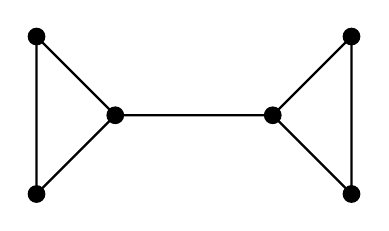
\begin{tikzpicture}
            \draw[fill=black] (0,0) circle (3pt);
            \draw[fill=black] (0,2) circle (3pt);
            \draw[fill=black] (1,1) circle (3pt);
            \draw[fill=black] (3,1) circle (3pt);
            \draw[fill=black] (4,0) circle (3pt);
            \draw[fill=black] (4,2) circle (3pt);
            \draw[thick] (1,1) -- (0,2) -- (0,0) -- (1,1) -- (3,1) -- (4,0) -- (4,2) -- (3,1);
        \end{tikzpicture}
        \caption{A graph with 6 vertices and 7 edges.} \label{fig-graph_example}
        \end{figure}
        
        From now on, we will skip $(G)$ and just write $V$ and $E$ if the context is obvious. Similarly we will skip $_G$ and just write $\sim$. Also, for simple graphs, we may write an edge as $vw$ where $v$ and $w$ are the ends of the edge.
        
        \begin{defn} \label{def_graph_terms} \begin{itemize}
            \item[]
            \item A vertex $v$ is \emph{adjacent} to another vertex $w$ if there is an edge $e$ such that $v \sim e$ and $w \sim e$. We also say that $v$ is a \emph{neighbor} of $w$.
            \item A \emph{loop} is an edge with exactly one end.
            \item Two edges $e_1$ and $e_2$ are \emph{parallel} if $e_1 \neq e_2$ and the set of ends of $e_1$ equals that of $e_2$.
            \item A graph $G$ is \emph{simple} if it has no loops or parallel edges.
            \item Two graphs $G$ and $H$ are \emph{isomorphic} if there are two bijections $f_V : V(G) \to V(H)$ and $f_E : E(G) \to E(H)$ such that for all $v \in V(G)$ and $e \in E(G)$, $v \sim_G e$ iff $f_V(v) \sim_H f_E(e)$.
        \end{itemize} \end{defn}
        
        Note that some texts might use a different definition of graphs. One common definition is that $E(G)$ is a set of two-element subsets of $V(G)$. With this definition, our definition of a simple graph is just called a graph, and our definition of a graph is called a multigraph.
        
        \begin{defn}[Subgraph] \label{def_subgraph} \begin{itemize}
            \item[]
            \item A graph $G$ is a \emph{subgraph} of a graph $H$ if $V(G) \subseteq V(H)$, $E(G) \subseteq E(H)$, with the same incidence relation, i.e. the set of ends of any edge $e$ in $G$ equals that of $e$ in $H$.
            \item For $e \in E$, $G \backslash e$ is $(V(G), E(G) \backslash \{e\})$ with the same incidence relation.
            \item For $v \in V$, $G \backslash v$ is $(V(G) \backslash \{v\}, E')$, where $E'$ is the set of edges in $G$ not incident with $v$, with the same incidence relation.
            \item A subgraph $H$ of $G$ is \emph{spanning} if $V(H) = V(G)$.
            \item A subgraph $H$ of $G$ is \emph{induced} if $E(H)$ equals the set of edges in $G$ whose set of ends is contained in $V(H)$. We say $H$ is \emph{induced by} $V(H)$.
            \item For $X \subseteq V$, $G[X]$ is a subgraph of $G$ induced by $X$.
        \end{itemize} \end{defn}
        
        \begin{defn} \label{def_graph_example} \begin{itemize}
            \item[]
            \item A \emph{complete graph} with $n$ vertices, denoted $K_n$, is a simple graph in which for any pair of different vertices there is an edge connecting them.
            \item A \emph{cycle graph} with $n$ vertices, denoted $C_n$, is a simple graph whose edge set is $\{v_1v_2, \cdots, v_{n-1}v_n, v_nv_1\}$, where $V = \{v_1, \cdots, v_n\}$.
            \item A graph $G$ is \emph{bipartite} if $V$ can be partitioned into non-empty subsets $A$ and $B$ such that no edges connect two vertices in $A$ or two vertices in $B$.
            \item A \emph{complete bipartite graph} with $n+m$ vertices, denoted $K_{n,m}$, is a simple bipartite graph with $|A|=n$, $|B|=m$ in which for any vertex in $A$ and in $B$, there is an edge connecting them.
            \item For a simple graph $G$, the \emph{complement} $\bar{G}$ of $G$ is a simple graph on $V(G)$ such that any two different vertices $v$ and $w$ are adjacent in $G$ iff they are not adjacent in $\bar{G}$.
        \end{itemize} \end{defn}
        
        \begin{figure}[h] \centering 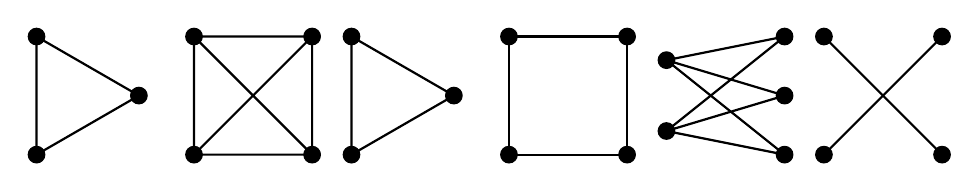
\begin{tikzpicture}
            % K3
            \draw[fill=black] (0,0) circle (3pt);
            \draw[fill=black] (0,1.5) circle (3pt);
            \draw[fill=black] (1.3,0.75) circle (3pt);
            \draw[thick] (0,0) -- (0,1.5) -- (1.3,0.75) -- (0,0);
            % K4
            \draw[fill=black] (2,0) circle (3pt);
            \draw[fill=black] (2,1.5) circle (3pt);
            \draw[fill=black] (3.5,0) circle (3pt);
            \draw[fill=black] (3.5,1.5) circle (3pt);
            \draw[thick] (2,0) -- (2,1.5) -- (3.5,1.5) -- (3.5,0) -- (2,0) -- (3.5,1.5) -- (3.5,0) -- (2,1.5);
            % C3
            \draw[fill=black] (4,0) circle (3pt);
            \draw[fill=black] (4,1.5) circle (3pt);
            \draw[fill=black] (5.3,0.75) circle (3pt);
            \draw[thick] (4,0) -- (4,1.5) -- (5.3,0.75) -- (4,0);
            % C4
            \draw[fill=black] (6,0) circle (3pt);
            \draw[fill=black] (6,1.5) circle (3pt);
            \draw[fill=black] (7.5,0) circle (3pt);
            \draw[fill=black] (7.5,1.5) circle (3pt);
            \draw[thick] (6,0) -- (6,1.5) -- (7.5,1.5) -- (7.5,0) -- (6,0);
            % K23
            \draw[fill=black] (8,0.3) circle (3pt);
            \draw[fill=black] (8,1.2) circle (3pt);
            \draw[fill=black] (9.5,0) circle (3pt);
            \draw[fill=black] (9.5,0.75) circle (3pt);
            \draw[fill=black] (9.5,1.5) circle (3pt);
            \draw[thick] (8,0.3) -- (9.5,0) -- (8,1.2) -- (9.5,0.75) -- (8,0.3) -- (9.5,1.5) -- (8,1.2);
            % C4 complement
            \draw[fill=black] (10,0) circle(3pt);
            \draw[fill=black] (10,1.5) circle(3pt);
            \draw[fill=black] (11.5,1.5) circle(3pt);
            \draw[fill=black] (11.5,0) circle(3pt);
            \draw[thick] (10,0) -- (11.5,1.5);
            \draw[thick] (10,1.5) -- (11.5,0);
        \end{tikzpicture}
        \caption{From left to right: $K_3$, $K_4$, $C_3$, $C_4$, $K_{2,3},$ and $\bar{C_4}$. Note that $K_3$ is isomorphic to $C_3$.} \label{fig-K3_K4}
        \end{figure}
        
        \begin{defn} \label{def_graph_path} \begin{itemize}
            \item[]
            \item A \emph{walk} from $v \in V$ and $w \in V$ is an alternating sequence $v_0 e_1 v_1 e_2 \cdots e_k v_k$ of vertices and edges such that $v_0 = v$, $v_k = w$, and the set of ends of $e_i$ equals $\{v_{i-1}, v_i\}$. $k$ is the \emph{length} of the walk.
            \item A \emph{trail} is a walk with distinct edges.
            \item A \emph{closed walk} is a walk with $v=w$ and $k>0$.
            \item A \emph{circuit} is a trail that is also a closed walk.
            \item A \emph{path} is a walk with distinct vertices.
            \item A \emph{cycle} is a circuit with distinct $\{v_0, \cdots, v_{k-1}\}$.
        \end{itemize} \end{defn}
        
        \begin{defn}[Connectivity] \label{def_connected_graph} \begin{itemize}
            \item []
            \item A graph is \emph{connected} if for any two vertices in $V$ there is a path connecting them.
            \item A \emph{connected component} of a graph $G$ is $G[X]$ such that $G[X]$ is connected, and for any $Y \subseteq V$ such that $X \subsetneq Y$, $G[Y]$ is not connected.
        \end{itemize} \end{defn}
    
    \section{Degrees}
    
        \begin{defn}[Degree] \label{def_graph_degree}
            The \emph{degree} of $v \in V(G)$, denoted $deg_G(v)$, is the number of non-loop edges incident with $v$, plus two times the number of loops incident with $v$.
        \end{defn}
        
        Again, we might skip $G$ and write $deg(v)$. As we progress, it will be clear why it is convenient to count a loop twice.
        
        \begin{lemma}[Degree Sum Formula] \label{lem_degree_sum}
            $\sum_{v \in V}deg(v) = 2|E|$.
        \end{lemma}
        
        \begin{proof}
            Induction on $|E|$, with the trivial base case $|E| = 0$. Suppose $|E| > 0$. Let $\sum_{v \in V}deg(v) = A$ and $2|E| = B$. Take any edge $e$, and the induction with $G\backslash e$ shows that $A-2 = B-2$. Therefore $A=B$.
        \end{proof}
        
        \begin{lemma}[Handshaking Lemma]
            A graph has an even number of odd-degree vertices.
        \end{lemma}
        
        \begin{proof}
            $2|E|$ is an even number. From [\ref{lem_degree_sum}], exactly even number of the terms $deg(v)$ must be odd.
        \end{proof}
        
        The degree sum formula is sometimes also called the handshaking lemma.
        
        \begin{defn}[Degree Sequence] \label{def_graph_score}
            The \emph{degree sequence} of a graph $G$, or the \emph{score} of $G$, is the sequence of degrees $(deg(v_1),\cdots,deg(v_{|V|}))$.
        \end{defn}
        
        Now, how can we figure out if a sequence is a degree sequence of some graph? The following theorem gives a simple $O(\sum d_i)$-time algorithm to answer the question:
        
        \begin{thm}[Havel-Hakimi Algorithm] \label{thm_havel_hakimi}
            Let $(d_1,\cdots,d_n)$ be a sequence of integers such that $0 \leq d_1 \leq \cdots \leq d_n$ and $n>1$. It is a degree sequence of some simple graph iff $(d_1,\cdots,d_{z-1},d_z-1,\cdots,d_{n-1}-1)$ is a degree sequence of some simple graph, where $z = n-d_n$.
        \end{thm}
        
        \begin{proof}
            ($\Leftarrow$) If $(d_1,\cdots,d_{z-1},d_z-1,\cdots,d_{n-1}-1)$ is a degree sequence of some simple graph, then we can make $(d_1,\cdots,d_n)$ by adding a vertex and connecting to the vertices with degrees $d_z-1,\cdots,d_{n-1}-1$.
            
            ($\Rightarrow$) Let $G$ be a simple graph such that $deg_G(v_i)=d_i$ for all $v_i \in V(G)$. We will construct a simple graph $H$ with $deg_H(u_i)=d_i$ for all $u_i \in V(H)$ such that $v_n$ is connected to $v_{n-d_n},\cdots,v_n-1$. Then the conclusion follows by taking $H-v_n$.
            
            If $d_n=n-1$, then simply take $H=G$. Otherwise, define $j(G)$ as the largest index $j$ such that $v_n$ is not adjacent to $v_j$. Among all graphs with $deg_H(u_i)=d_i$, take one graph with the smallest $j(H)$. (Note that such $H$ exists because at least one graph, namely $G$, satisfies the degree sequence condition.)
            
            Suppose $j=j(H) \geq n-d_n$. Then there is an index $i<j$ such that $u_n$ is adjacent to $u_i$. Since $deg_H(u_i) \leq deg_H(u_j)$, there is a vertex $w$ adjacent to $u_j$ but not to $u_i$. Now, consider a new graph $H'$ derived from $H$ by removing $u_iu_n$ and $u_ju_k$, and adding $u_ju_n$ and $u_iu_k$. Then $deg_{H'}(u_i)=d_i$ and $j(H')<j(H)$, contradicting the minimality of $H$. Therefore $j(H) = n-d_n$.
        \end{proof}
    
    \section{Trees}
        One of the important classes of graphs is a tree. There are many ways to define a tree. First we will state one definition, and then prove that other definitions are equivalent.
        \begin{defn}[Tree] \label{def_tree}
            A \emph{forest} is a simple graph without any cycle. A \emph{tree} is a connected forest. A \emph{leaf} of a forest is a vertex with degree 1.
        \end{defn}
        
        \begin{thm} \label{thm_tree}
            The following statements are equivalent for a simple graph $G$: \begin{enumerate}
                \item $G$ is a tree.
                \item For any two vertices $u$ and $v$ of $G$, there is exactly one path connecting them.
                \item $G$ is connected, and for any $e$ of $G$, $G \backslash e$ is disconnected.
                \item $G$ has no cycle, and for any two vertices $u$ and $v$ not having an edge between them, $G+uv$ has a cycle.
                \item $G$ is connected, and $|E| = |V|-1$.
            \end{enumerate}
        \end{thm}

        \begin{proof}
            TODO
            %(1 $\Rightarrow$ 4) $T$ has no cycles. For any $x,y \in V$, there is a path from $y$ to $x$. That path and $xy$ creates a cycle in $T+xy$.
            
            %(4 $\Rightarrow$ 3) For any $x,y \in V$, $T+xy$ has a cycle and that cycle must contain $xy$. Removing $xy$ from the cycle yields a path from $x$ to $y$. Therefore $T$ is connected. Now suppose $T \backslash e$ is connected for some $e \in E$, and $e$ connects $x$ and $y$. There is a path from $y$ to $x$ in $T \backslash e$, and that path and $e$ creates a cycle in $T$: contradiction.
            
            %(3 $Righatrrow$ 2) $G$ is connected.
        \end{proof}
        
        \begin{thm} \label{thm_tree_leaf}
            A tree with at least 2 vertices has at least 2 leaves.
        \end{thm}
        
        \begin{proof}
            From [\ref{thm_tree}](5) and [\ref{lem_degree_sum}], the sum of degrees is $2|V|-2$. None of the degrees are 0. Therefore at least 2 degrees must equal 1.
        \end{proof}
        
        How can we figure out if a sequence is a degree sequence of some tree? It turns out to be a lot simpler than [\ref{thm_havel_hakimi}] and basically anything that makes sense can be a degree sequence of a tree:
        
        \begin{thm}[Degree Sequence of a Tree] \label{thm_tree_degree}
            A sequence $(d_1,\cdots,d_n)$ is a degree sequence of some tree iff all $d_i$ are positive and $\sum d_i = 2n-2$.
        \end{thm}
        
        \begin{proof}
            ($\Rightarrow$) Clear from [\ref{thm_tree}](5) and [\ref{lem_degree_sum}].
            
            ($\Leftarrow$) Induction on $n$, with trivial base cases $n \leq 2$. Now suppose $n \geq 3$. There exists $i$ and $j$ such that $d_i=1$ and $d_j>1$; WLOG assume $i=1$ and $j=2$. From induction, $(d_2-1,d_3,\cdots,d_n)$ is a degree sequence of some tree. Take any vertex $v$ in the tree with degree $d_2-1$, and add a leaf adjacent to $v$. This constructs a tree with the degree sequence $(d_1,\cdots,d_n)$.
        \end{proof}
    
    \subsection{Spanning Trees}
        \begin{defn}[Spanning Subgraph] \label{def_spanning}
            A \emph{spanning subgraph} of a graph $G$ is a subgraph of $G$ such that its vertex set equals $V(G)$. A \emph{spanning tree} is a spanning graph that is a tree.
        \end{defn}
        
        \begin{thm} \label{thm_spanning_tree}
            A connected graph $G$ has a spanning tree.
        \end{thm}
        
        \begin{proof}
            Let $m = |E|$, and label the edges as $e_0$, $\cdots$, $e_m$, arbitrarily. Define the subsets $E_0$, $\cdots$, $E_m$ of $E$, as \begin{displaymath} \begin{cases}
                E_0 = \varnothing \\
                E_i = E_{i-1} \cup \{e_i\} & \text{if the spanning subgraph of $G$} \\
                & \text{with $E = E_{i-1} \cup \{e_i\}$ has no cycle} \\
                E_i = E_{i-1} & \text{otherwise.}
            \end{cases} \end{displaymath}
            Let $H$ be the spanning subgraph of $G$ with $E = E_m$. Clearly, $H$ has no cycle. If $e_i \notin E_m$ and $H+e_i$ has no cycle, then $E_i$ would contain $e_i$, contradiction. From [\ref{thm_tree}], $H$ is a tree.
        \end{proof}
        
        (TODO: minimum spanning tree)
        
        There are other minimum spanning tree algorithms like Prim's algorithm or Borůvka's algorithm.
    
    \section{Planar Graphs}
        \begin{defn}[Planar Graph] \label{def_planar_graph}
            A \emph{plane graph} is a graph $G$ where: \begin{itemize}
                \item $V \subseteq \mathbb{R}^2$;
                \item every edge is an arc between two endpoints;
                \item the interior of each edge contains no vertex and no point of any other edge.
            \end{itemize}
            The connected components of $\mathbb{R}^2 \backslash G$ are called \emph{faces} of $G$. Since $G$ is contained in a sufficiently large disc, exactly one face is unbounded; that face is called the \emph{outer face} of $G$. All other faces are called \emph{inner faces} of $G$. A graph $H$ is \emph{planar} if it is isomorphic to some plane graph.
        \end{defn}
        
        \begin{thm}[Euler's Formula] \label{thm_euler_vef}
            If $G$ is a connected plane graph, and the number of faces of $G$ is $F$, then \begin{displaymath}
                |V| - |E| + F = 2.
            \end{displaymath}
        \end{thm}
        
        \begin{proof}
            Induction on $|E|$. The base case is when $G$ has no edges, one vertex, and one face; the formula clearly holds.
            
            Pick any edge $e$. If $e$ is a loop, removing it reduces $|E|$ and $F$ by one. Otherwise, contracting it reduces $|V|$ and $|E|$ by one. Either way the result follows by induction.
        \end{proof}
        
        \begin{thm} \label{thm_planar_ve}
            If $G$ is simple and planar, and $|V| \geq 3$, then $|E| \leq 3|V|-6$. If in addition $G$ has no triangles (i.e. $K_3$ as a subgraph), then $|E| \leq 2|V|-4$.
        \end{thm}
        
        \begin{proof}
            Count the number $N$ of pairs $(f, e)$ where the face $f$ and the edge $e$ are incident. For each face, there are at least 3 edges incident to it, for otherwise there would be parallel edges or loops. Therefore $N \geq 3F$. On the other hand, each edge is incident to exactly two faces, so $N = 2|E|$. This gives $3F \leq 2|E|$. From [\ref{thm_euler_vef}], $3F = 6-3|V|+3|E| \leq 2|E|$, and the first result follows.
            
            The second result can be proved in the exactly same way, using $N \geq 4F$.
        \end{proof}
        
        \begin{coro} \label{cor_k5_k33}
            $K_5$ and $K_{3,3}$ are not planar.
        \end{coro}
        
        \begin{proof}
            $K_5$ has 5 vertices and 10 edges. $K_{3,3}$ has no triangles, 6 vertices, and 9 edges. The result follows from [\ref{thm_planar_ve}].
        \end{proof}
        
        TODO: add a figure of K5 and K33.
        
        It clearly follows that any subdivision of $K_5$ or $K_{3,3}$ are not planar. Surprisingly, those two graphs are the only graphs that ``need to be checked" to determine if a given graph is planar. The proof requires several more lemmas and theorems, so we have moved the proof to the appendix.
        
        \begin{thm}[Kuratowski's Theorem] \label{thm_kuratowski}
            A graph $G$ is planar if and only if it does not have $K_5$ or $K_{3,3}$ as a topological minor.
        \end{thm}
    
    \section{Coloring}
        \begin{defn}[Coloring] \label{def_coloring}
            A \emph{$k$-coloring} of a graph $G$ is a function $c: V(G) \to \{1,2,\cdots,k\}$ such that if $u$ and $v$ are adjacent vertices, then $c(u) \neq c(v)$. $G$ is \emph{$k$-colorable} if there is a $k$-coloring of $G$. The \emph{chromatic number} $\chi(G)$ of $G$ is the smallest integer $k$ such that $G$ is $k$-colorable.
        \end{defn}
        
        Perhaps the most famous theorem about graph coloring is the four-color theorem. (TODO: write something) 
        
        \begin{thm}[Four-color Theorem] \label{thm_four_color}
            If $G$ is planar, then $\chi(G) \leq 4$.
        \end{thm}
        
        Unfortunately, the proof is too long and complicated to contain in the codex. We prove a weaker result:
        
        \begin{thm}[Five-color Theorem] \label{thm_five_color}
            If $G$ is planar, then $\chi(G) \leq 5$.
        \end{thm}
        
        \begin{proof}
            Induction on $|V|$. For $|V| \leq 5$, the theorem is trivial.
            
            From [\ref{thm_planar_ve}], $G$ has a vertex $v$ of degree at most 5. If $deg_G(v) < 5$, then inductively find a 5-coloring of $G-v$, and color $v$ by some color in $\{1,2,3,4,5\}$ not appearing in the neighbors of $v$. If $deg_G(v) = 5$ and not all colors are used in the neighbors of $v$, then the same argument applies.
            
    \begin{figure}[h] \centering 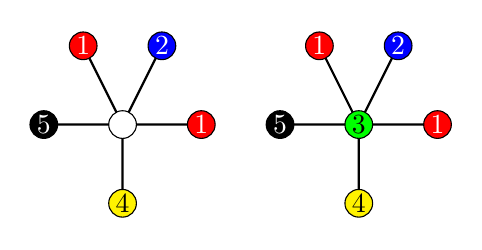
\begin{tikzpicture}
        \draw[thick] (0,0) -- (-0.5,1) -- (0,0) -- (0.5,1) -- (0,0) -- (1,0) -- (0,0) -- (0,-1) -- (0,0) -- (-1,0);
        \draw[fill=white] (0,0) circle (5pt);
        \draw[fill=red] (-0.5,1) circle (5pt);
        \node[white] at (-0.5,1) {1};
        \draw[fill=blue] (0.5,1) circle (5pt);
        \node[white] at (0.5,1) {2};
        \draw[fill=red] (1,0) circle (5pt);
        \node[white] at (1,0) {1};
        \draw[fill=yellow] (0,-1) circle (5pt);
        \node at (0,-1) {4};
        \draw[fill=black] (-1,0) circle (5pt);
        \node[white] at (-1,0) {5};
        
        \draw[thick] (3,0) -- (2.5,1) -- (3,0) -- (3.5,1) -- (3,0) -- (4,0) -- (3,0) -- (3,-1) -- (3,0) -- (2,0);
        \draw[fill=green] (3,0) circle (5pt);
        \node at (3,0) {3};
        \draw[fill=red] (2.5,1) circle (5pt);
        \node[white] at (2.5,1) {1};
        \draw[fill=blue] (3.5,1) circle (5pt);
        \node[white] at (3.5,1) {2};
        \draw[fill=red] (4,0) circle (5pt);
        \node[white] at (4,0) {1};
        \draw[fill=yellow] (3,-1) circle (5pt);
        \node at (3,-1) {4};
        \draw[fill=black] (2,0) circle (5pt);
        \node[white] at (2,0) {5};
    \end{tikzpicture}
    \end{figure}
            
            Now suppose all 5 colors are used. Denote the neighbors of $v$ as $u_1$, $u_2$, $u_3$, $u_4$, $u_5$, in clockwise order. Without loss of generality, we will assume that $c(u_i)=i$.
            
            The main idea of the rest of the proof is that we want to change the color of one of the neighbors, say change $c(u_i)$ to $k$. This is impossible if $u_i$ has a neighbor of color $k$, in which case we want to also change the color of that neighbor, to $k'$. But then that neighbor might have yet another neighbor of color $k'$, and this continues to form a chain. Hence we introduce the \emph{Kempe chain}, named after Alfred Kempe.
            
            Let $V_{ij}$ be the set of vertices $w$ in $G$ such that there is a path from $u_i$ to $w$ consisting of vertices of color $i$ or $j$. Note that if we switch the colors of the vertices in $V_{ij}$ (i.e. change $i$ to $j$ and $j$ to $i$), and leave everything else the same, then the result is still a coloring.
            
            If $V_{13}$ does not contain $u_3$, then switch the colors of the vertices in $V_{13}$ and color $v$ by 1.
            
            (TODO: picture)
            
            Otherwise, $V_{24}$ does not contain $u_4$; switch the colors of the vertices in $V_{24}$ and color $v$ by 2. This gives a 5-coloring of $G$.
            
            (TODO: picture)
        \end{proof}
        
        Fun fact: In 1879, the Kempe chain method was used to ``prove" the four-color theorem by Alfred Kempe. No one noticed that this ``proof" had an error until eleven years later when Percy Heawood found the error. What we saw above is the modification of the incorrect proof to prove the weaker theorem. The correct proof of four-color theorem was completed in 1976 by Kenneth Appel and Wolfgang Haken.
        
        Here is his ``proof." Argue similarly as above with induction. If $deg_G(v) = 4$ and all 4 colors are used, then apply the Kempe chain method. Now suppose $deg_G(v) = 5$ and all 4 colors are used. Then one color is used exactly twice.
        
        There are two cases: the two neighbors with that color are next to each other in clockwise order, or they are not. The first case is easy, just use the Kempe chain method. The second case is where the fun starts.
        
        (TODO: picture. u5-u4-u1-u2-u3 clockwise; u1 and u5 has the same color. Cetner is noted v.)
        
        WLOG, $u_k$ has color $k$. For convenience, color 5 is the same as color 1.
        
        If $V_{42}$ does not contain $u_2$, then switch the colors of the vertices in $V_{25}$ and color $v$ by 4. Otherwise, if $V_{43}$ does not contain $u_3$, then switch and color $v$ by 4. Otherwise, $V_{13}$ does not contain $u_3$ and $V_{52}$ does not contain $u_2$. Switch each chain and color $v$ by 1.
        
        (TODO: second case picture.)
        
        Can you find a critical error in this argument? If you want to know, refer to the appendix.
    
\end{document}